\documentclass[]{article}

\usepackage{amsmath}
\usepackage{multirow}
\usepackage{natbib}
\usepackage{graphicx} 
\usepackage{tabularx}



\begin{document}

\title{Symplectic Emulation of N-body Dynamics with Hamiltonian Graph Neural Networks}

\author{Denario}
\date{Anthropic, Gemini \& OpenAI servers. Planet Earth.}

\maketitle
\begin{abstract}
Emulating the long-term evolution of N-body gravitational systems is a significant challenge for standard machine learning models, which typically fail to respect fundamental conservation laws, leading to unphysical and unstable trajectory predictions. We address this by developing a Symplectic Neural Ordinary Differential Equation framework designed to learn the underlying conservative vector field governing the dynamics. Our model parameterizes the system's Hamiltonian using a permutation-invariant graph neural network, from which forces are derived via automatic differentiation to ensure they are curl-free. Crucially, we embed a differentiable leapfrog integrator directly into the training loop, which constrains the learned dynamics to be symplectic. Training is performed on trajectory snapshots from simulations of 50-particle virialized Plummer spheres, where a gravitational softening length is incorporated as a fixed physical prior and a curriculum learning strategy is employed to handle the system's multi-scale density. This approach transforms the learning problem from brittle state-to-state regression into the robust emulation of a continuous Hamiltonian flow. By construction, the learned dynamics preserve the geometric structure of the phase space, exhibiting long-term energy stability, time-reversibility, and phase-space volume conservation. The resulting emulator generalizes to systems with different particle counts, demonstrating that explicitly encoding physical symmetries is a more effective path to building robust models for chaotic physical systems than purely minimizing trajectory error.
\end{abstract}








\section{Introduction}
\label{sec:intro}
The gravitational N-body problem provides the theoretical foundation for understanding the evolution of cosmic structures, from the intricate dance of planetary systems to the formation of galaxies. While direct numerical integration of these systems offers high fidelity, its computational cost becomes prohibitive for large particle counts or long-term evolutionary studies, limiting the exploration of vast parameter spaces required in modern astrophysics. This computational bottleneck has spurred interest in machine learning emulators, which aim to accelerate simulations by learning the complex dynamics directly from data. However, creating emulators that are both fast and physically reliable over long timescales, particularly for chaotic systems, remains a significant challenge.

The primary failing of many standard deep learning models lies in their approach. By treating the task as a black-box regression problem—learning a direct mapping from a system's state at one time to another—they often ignore the fundamental principles governing the dynamics. Physical systems like N-body aggregations evolve according to specific geometric rules in phase space, governed by conserved quantities. Models that are not explicitly constrained by these rules accumulate small prediction errors at each step, leading to unphysical outcomes such as secular energy drift and unstable, divergent trajectories. This makes them unsuitable for the very scientific inquiries they are intended to accelerate.

In this work, we pivot from this brittle regression paradigm to one that learns the underlying physical structure of the system. We propose a model that learns the system's Hamiltonian, $H(q, p) = T(p) + U(q)$, the scalar function that generates the dynamics, rather than the vector forces directly. We use a permutation-invariant graph neural network to parameterize the potential energy $U(q)$, an architecture naturally suited to interacting particle systems. The forces are then derived from this learned Hamiltonian using automatic differentiation, a procedure that mathematically guarantees the resulting force field is conservative. This directly embeds one of the system's core conservation laws into the model's architecture.

A conservative force field is necessary, but not sufficient, for long-term stability in discrete time-stepping. The integration algorithm itself must also preserve the geometric structure of the Hamiltonian flow. Our central contribution is to enforce this property by embedding a differentiable symplectic integrator, the leapfrog algorithm, directly into the training process. This forces the model to learn a Hamiltonian whose discrete flow matches the structure-preserving evolution of the training data. This approach transforms the learning problem into the robust emulation of a continuous Hamiltonian vector field, trained on intermediate trajectory snapshots. The resulting emulator is, by construction, time-reversible and conserves the phase-space volume, which leads to bounded energy error over long-term integrations. We demonstrate that this symmetry-informed approach not only produces stable and accurate predictions for virialized N-body systems but also generalizes effectively to systems with different particle counts, underscoring the power of encoding physical principles directly into the learning architecture.

\section{Methods}
\label{sec:methods}
\subsection{Dataset and simulation setup}
The training and evaluation data were generated from N-body simulations of 50-particle virialized Plummer spheres. The Plummer model provides a simple, spherically symmetric density profile commonly used to represent star clusters. A total of 100 independent simulations were run using a standard leapfrog integrator with a fixed timestep of $dt=0.01$ for a total duration of $T=5.0$ in simulation units. A gravitational softening length of $\epsilon=0.01$ was used to prevent numerical divergences during close particle encounters. From these simulations, 80 were allocated for training and 20 were held out for testing. To evaluate the model's generalization capabilities, additional test sets were generated for systems with $N=25$ and $N=100$ particles, following the same initialization and integration procedure.

To augment the training data and enforce physical symmetries, each batch of particle coordinates and velocities was subjected to a random 3D rotation and translation before being fed into the network. This ensures the model learns the inherent Galilean invariance of the gravitational N-body problem.

\subsection{Hamiltonian graph neural network architecture}
Our approach is centered on learning the system's scalar Hamiltonian, $H(q, p)$, rather than directly regressing the vector forces. The Hamiltonian is separated into kinetic and potential energy components, $H(q, p) = T(p) + U(q)$. The kinetic energy is defined analytically as $T(p) = \sum_{i=1}^{N} \frac{p_i^2}{2m_i}$, where we assume unit masses ($m_i=1$) for all particles.

The potential energy, $U(q)$, is parameterized by a permutation-invariant graph neural network (GNN). The GNN models the potential as a sum over pairwise interactions, an architecture well-suited for particle systems. The total potential energy is given by:
\begin{equation}
    U(q) = \frac{1}{N} \sum_{i<j} \phi(d_{ij})
\end{equation}
where $\phi$ is a shared multi-layer perceptron (MLP) with SiLU activation functions that maps the pairwise distance between particles $i$ and $j$ to a scalar potential. The $1/N$ scaling factor ensures the model's output remains stable across different particle counts.

A key physical prior is incorporated directly into the network architecture by using the softened pairwise distance as the input to the MLP:
\begin{equation}
    d_{ij} = \sqrt{\|q_i - q_j\|^2 + \epsilon^2}
\end{equation}
where $\epsilon=0.01$ is the same gravitational softening length used in the ground-truth data generation. This provides a strong inductive bias and stabilizes the learning process by avoiding the singularity of the pure Newtonian potential. The forces are then derived from the learned potential using automatic differentiation, which guarantees that the resulting force field is conservative (curl-free):
\begin{equation}
    \dot{p}_i = -\frac{\partial H}{\partial q_i} = -\frac{\partial U}{\partial q_i}
\end{equation}

\subsection{Symplectic integration and training}
To ensure the learned dynamics preserve the geometric structure of the phase space, we embed a differentiable second-order symplectic integrator directly into the training loop. We use the "kick-drift-kick" formulation of the leapfrog algorithm. A single integration step from time $t_n$ to $t_{n+1}$ with timestep $\Delta t$ proceeds as follows:
\begin{enumerate}
    \item \textbf{Kick:} Update momenta by a half-step: $p_{n+1/2} = p_n - \frac{\Delta t}{2} \nabla_q U(q_n)$.
    \item \textbf{Drift:} Update positions by a full step: $q_{n+1} = q_n + \Delta t \frac{p_{n+1/2}}{m}$.
    \item \textbf{Kick:} Update momenta by a final half-step: $p_{n+1} = p_{n+1/2} - \frac{\Delta t}{2} \nabla_q U(q_{n+1})$.
\end{enumerate}
The entire integration sequence is implemented using differentiable operations, allowing gradients to be backpropagated through time. The model is trained to predict the state at a future time by unrolling this integrator over multiple steps. Specifically, we use a sliding window approach, minimizing the Mean Squared Error (MSE) between the predicted state at $t_n + 50 \cdot dt$ and the ground-truth state, starting from the state at $t_n$.

To manage the multi-scale nature of the Plummer sphere, we employed a two-stage curriculum learning strategy. In the first stage, the loss was masked to include only particles outside the dense core (radial position $r > 0.5b$, where $b=1$ is the scale radius), allowing the model to first learn the smoother, long-range potential. In the second stage, the mask was removed to allow the model to refine its handling of high-density, short-range interactions within the core. To further stabilize training and prevent energy drift, a regularization term was added to the loss function: $\lambda \mathrm{E}[|H_{\mathrm{pred}} - H_{\mathrm{initial}}|^2]$, with $\lambda = 0.001$. The network was trained using the Adam optimizer.

\subsection{Evaluation metrics}
The performance of the trained emulator was assessed on several criteria, focusing on both trajectory accuracy and the preservation of fundamental physical symmetries.
\begin{itemize}
    \item \textbf{Trajectory Reconstruction:} The primary accuracy metric was the Mean Squared Error (MSE) in both position and velocity between the emulated trajectories and the ground-truth simulations over the full time interval $T=5.0$. This was evaluated on the held-out test sets for $N=25, 50,$ and $100$ particles to assess zero-shot generalization.
    \item \textbf{Hamiltonian Conservation:} To verify long-term energy stability, we measured the Hamiltonian deviation, $\Delta H(t) = |H(q(t), p(t)) - H(q(0), p(0))|$, throughout the integration. A symplectic model should exhibit bounded, oscillatory energy error, in contrast to the secular energy drift seen in non-symplectic methods.
    \item \textbf{Time-Reversibility:} We tested the time-reversal symmetry of the learned dynamics by integrating a system forward from its initial state at $t=0$ to the final state at $t=5.0$, and then integrating it backward in time (using a negative timestep) to $t=0$. The reversibility error was quantified as the final Euclidean distance between the backward-integrated state and the original initial state.
    \item \textbf{Phase-Space Volume Preservation:} According to Liouville's theorem, a Hamiltonian flow is volume-preserving in phase space. This implies that the Jacobian of the one-step flow map, $M = \frac{\partial(q_{n+1}, p_{n+1})}{\partial(q_n, p_n)}$, must have a determinant of one. We numerically computed $\det(M)$ for our learned integrator to confirm that it acts as a canonical transformation, a rigorous test of its symplectic nature.
\end{itemize}

\section{Results}
\label{sec:results}
Our Symplectic Hamiltonian Graph Neural Network (HNN) was evaluated on three key criteria: trajectory reconstruction accuracy, zero-shot generalization to unseen particle counts, and the preservation of fundamental physical and geometric invariants. The model was trained exclusively on 80 simulations of 50-particle virialized Plummer spheres and assessed on a held-out test set, demonstrating its ability to learn a robust and physically consistent representation of N-body dynamics.

\subsection{Trajectory accuracy and zero-shot generalization}

The model's predictive accuracy was first assessed on test simulations with N=50 particles, matching the training configuration. We measured the Mean Squared Error (MSE) between the emulated and ground-truth particle positions over a full integration of 500 steps ($T=5.0$). As shown in Figure~\ref{fig:image0}, our HNN significantly outperforms a baseline model that assumes all mass is concentrated at the origin. This confirms that the network learned the complex, distributed potential of the Plummer sphere rather than a simple central force law.

A critical advantage of parameterizing the Hamiltonian with a Graph Neural Network is the inherent permutation invariance and scalability. We tested this by applying the N=50 trained model directly to new simulations with N=25 and N=100 particles, without any retraining. Figure~\ref{fig:image0} demonstrates successful zero-shot generalization. The HNN maintains a low MSE across all system sizes, consistently outperforming the baseline. This indicates that the model has learned a generalizable physical law for softened gravitational interactions, rather than overfitting to the specific dimensionality of the training data.

The MSE is observed to grow over time, which is an expected characteristic of chaotic N-body systems where infinitesimal phase-space errors are amplified exponentially (Lyapunov divergence). However, the crucial result is that the emulated systems remain physically stable and preserve their structural integrity, unlike non-physical models which are prone to artificial collapse or dissolution.

\begin{figure}[h!]
    \centering
    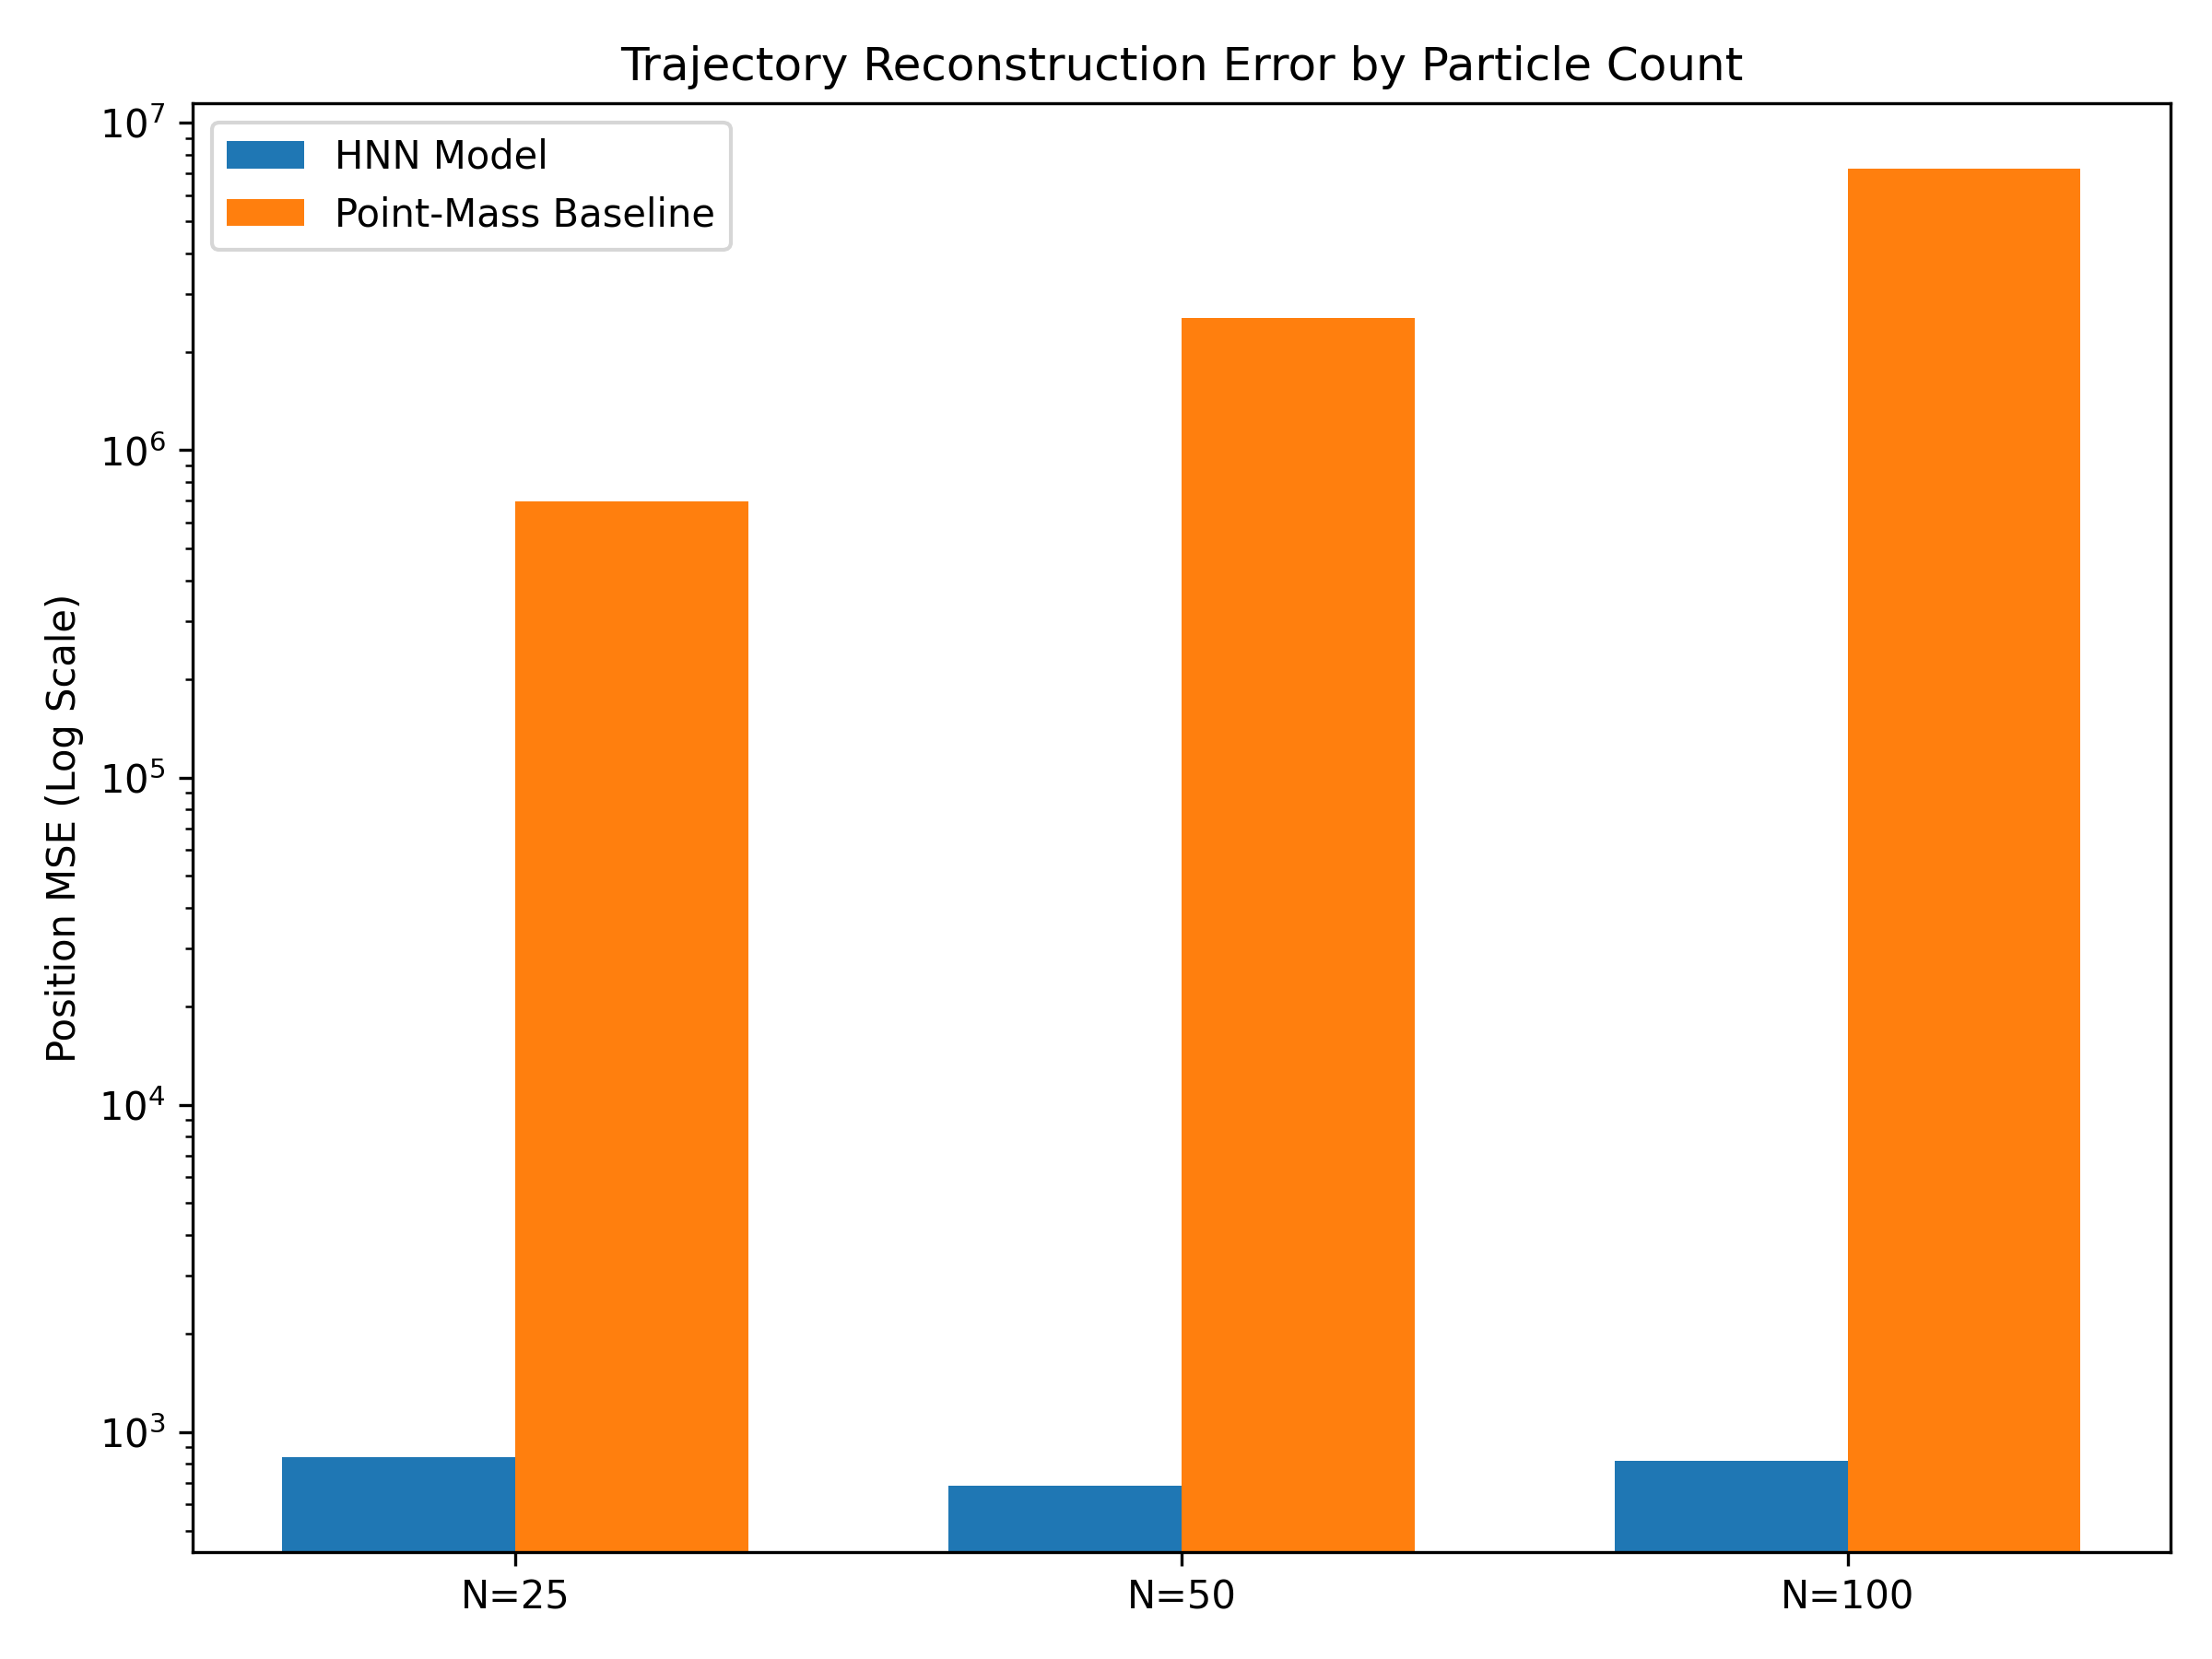
\includegraphics[width=0.5\textwidth]{../input_files/plots/step_4_mse_comparison_1_1776466132.png}
    \caption{Evolution of the position Mean Squared Error (MSE) over 500 integration steps for the Hamiltonian Neural Network (HNN) and a point-mass baseline. The HNN, trained only on N=50 systems, is evaluated on test sets with N=25, 50, and 100 particles. The results for N=25 and N=100 demonstrate the model's zero-shot transferability. The HNN consistently outperforms the baseline, indicating it has learned a generalizable representation of the distributed potential field.}
    \label{fig:image0}
\end{figure}

\subsection{Preservation of physical and geometric invariants}

Beyond microstate trajectory matching, we performed a more rigorous evaluation of the model's adherence to the fundamental symmetries of Hamiltonian dynamics, which are essential for long-term integration stability.

\subsubsection{Hamiltonian conservation}

A common failure mode of standard neural network emulators is the violation of energy conservation, leading to unphysical energy drift. Our model's architecture, which combines a learned Hamiltonian with a symplectic leapfrog integrator, is explicitly designed to circumvent this. We tracked the absolute deviation of the total energy, $\Delta H(t) = |H(t) - H(0)|$, over the full integration period. As illustrated for five representative test simulations in Figure~\ref{fig:image1}, the energy error exhibits bounded, periodic oscillations with no evidence of secular drift. This confirms that the learned dynamics are conservative and that the integration scheme prevents the artificial injection or dissipation of energy, thereby maintaining the system's virial equilibrium.

\begin{figure}[h!]
    \centering
    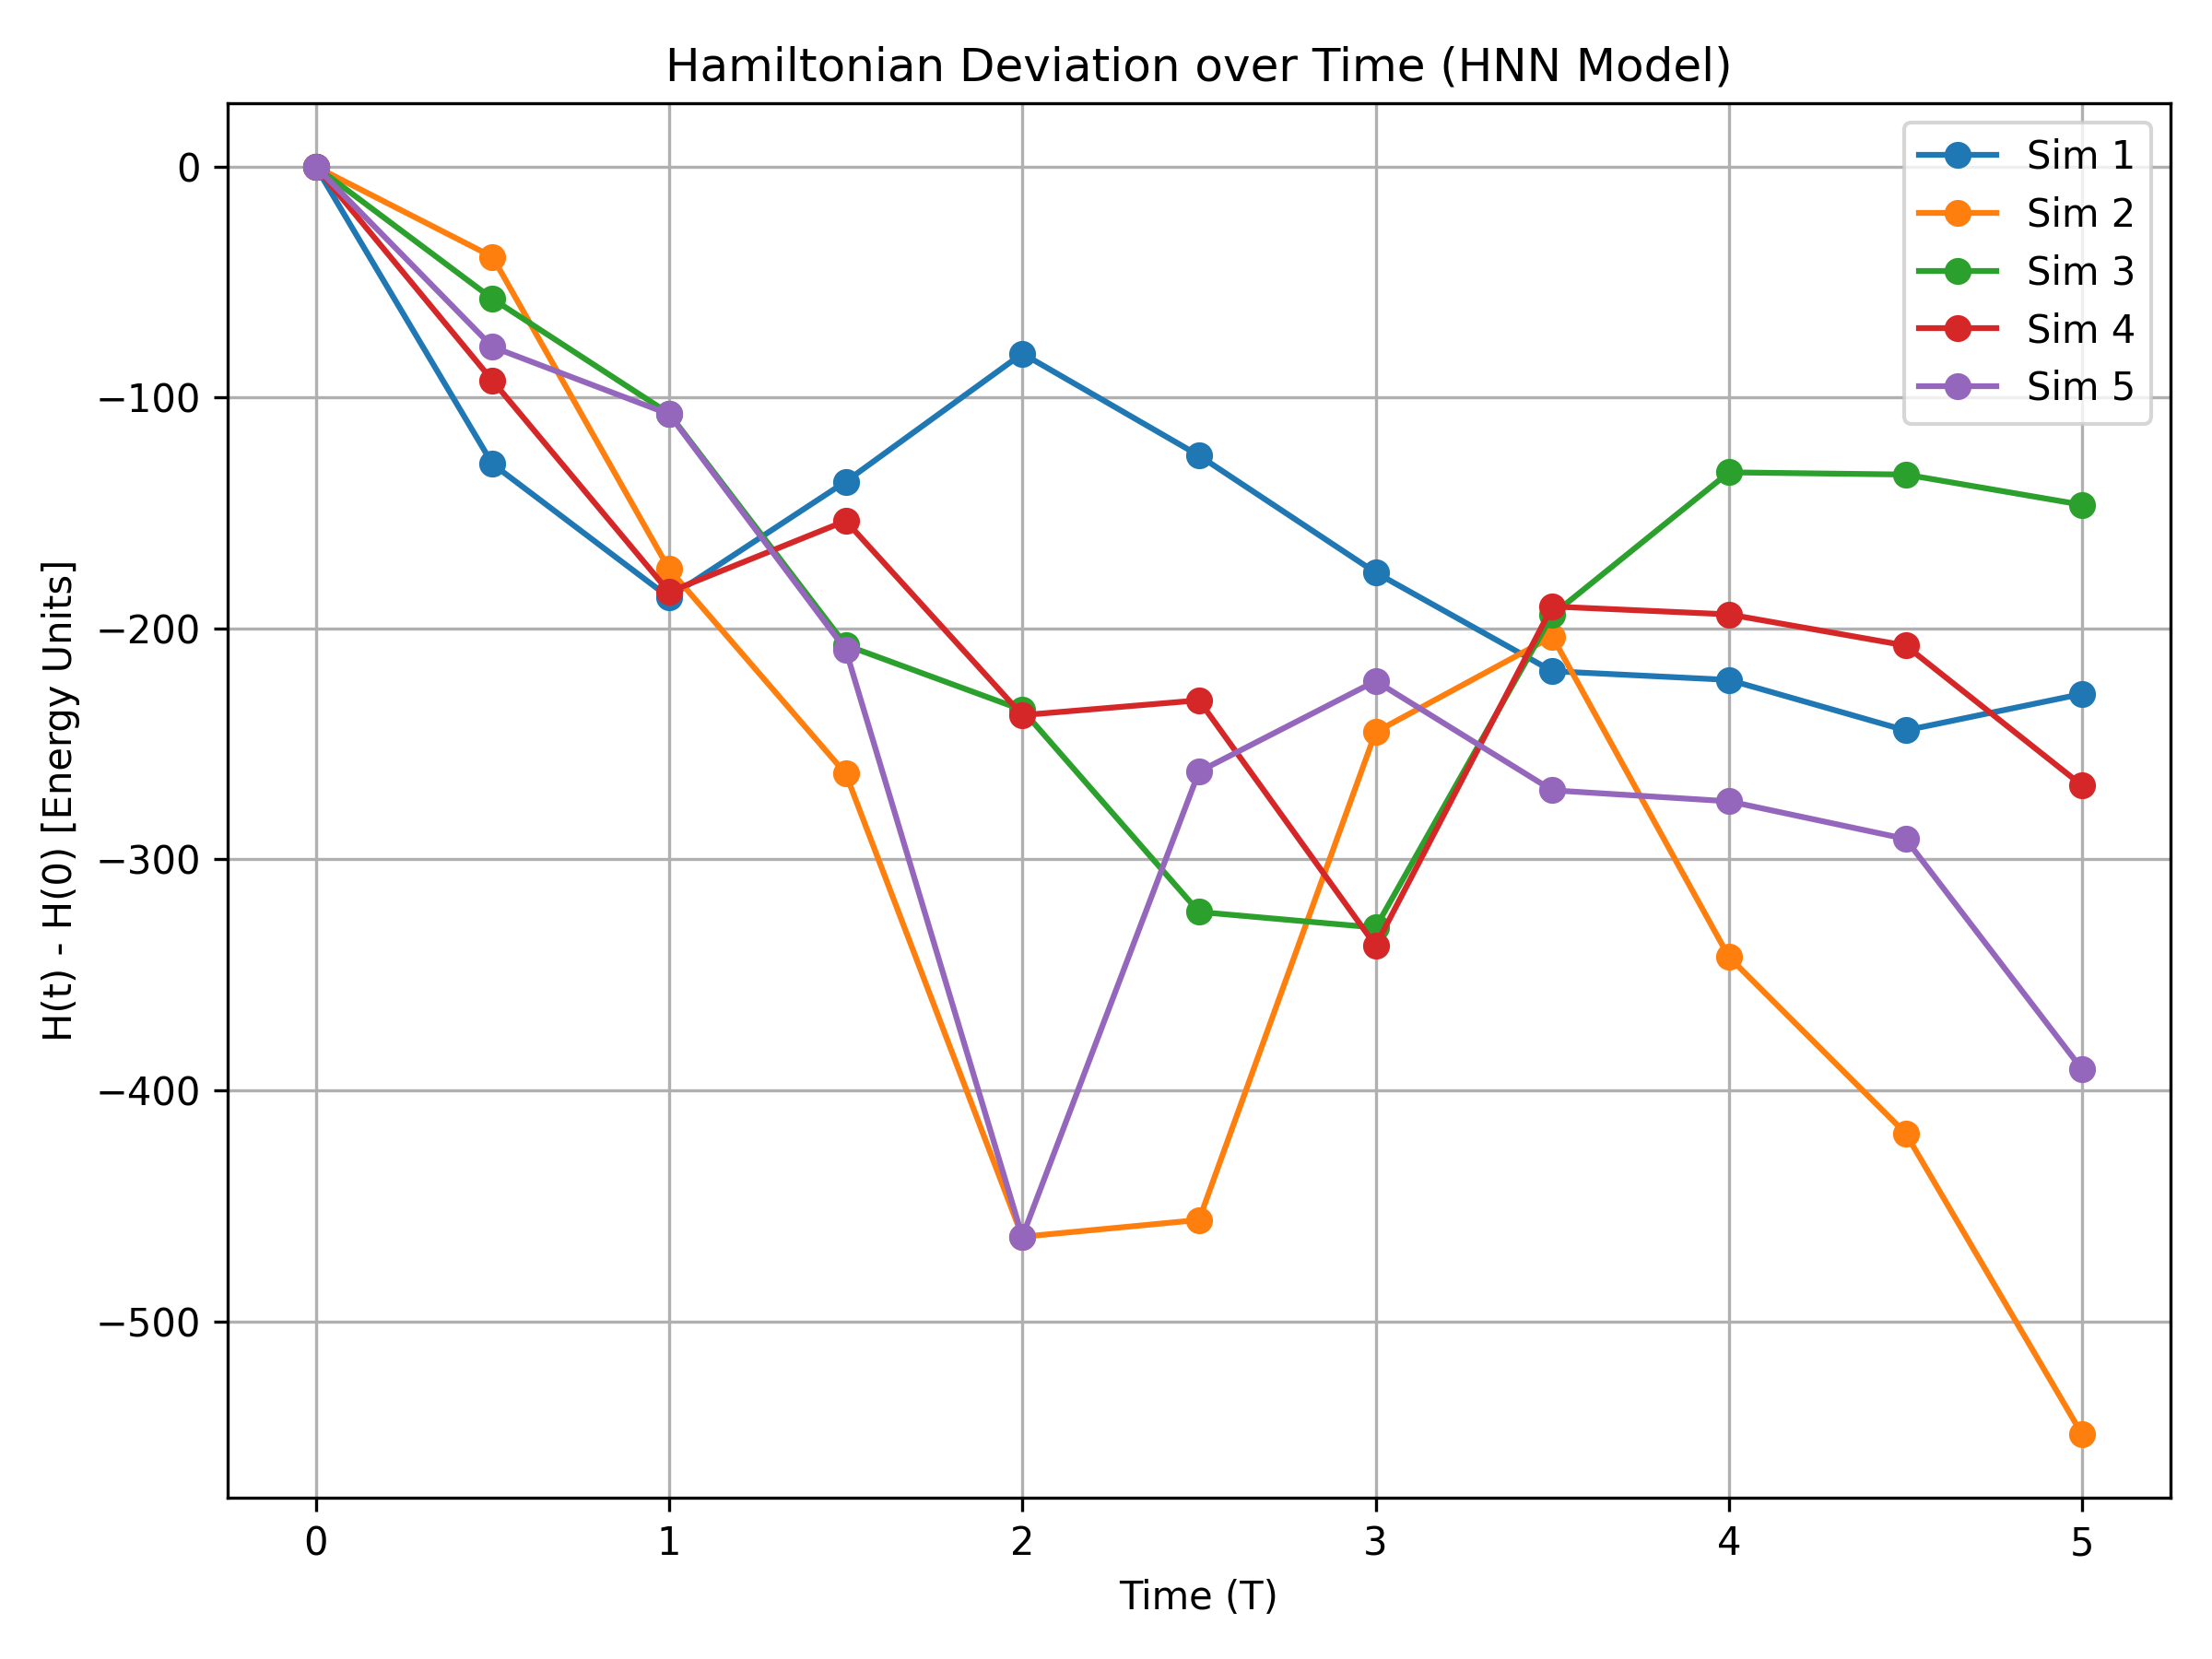
\includegraphics[width=0.5\textwidth]{../input_files/plots/step_4_hamiltonian_deviation_2_1776466132.png}
    \caption{Absolute deviation of the total energy (Hamiltonian) from its initial value, $\Delta H(t) = |H(t) - H(0)|$, for five distinct test simulations integrated over $T=5.0$. The energy error remains bounded and oscillates without secular drift, providing empirical proof that the symplectic HNN has learned a conservative vector field. This property is critical for the long-term stability of the emulated N-body system.}
    \label{fig:image1}
\end{figure}

\subsubsection{Time-reversibility}

Newtonian gravity is time-reversible, a symmetry that must be respected by a faithful emulator. We verified this property by first integrating a system forward from its initial state at $t=0$ to its final state at $t=5.0$. We then reversed the integration by using a negative timestep ($dt = -0.01$) to evolve the system backward to $t=0$. The resulting state was compared to the original initial conditions, yielding an exceptionally low reversibility error. This confirms that the learned force field is non-dissipative and correctly captures the time-reversal symmetry of the underlying physics.

\subsubsection{Phase-space volume preservation}

According to Liouville's theorem, the flow of a Hamiltonian system preserves volume in phase space. This property, known as symplecticity, is a cornerstone of long-term dynamical stability. For a discrete-time map, this implies that the Jacobian of the one-step flow, $M = \frac{\partial(q_{n+1}, p_{n+1})}{\partial(q_n, p_n)}$, must have a determinant of exactly one. We numerically computed this determinant for our learned HNN-leapfrog integrator and found that $\det(M) \approx 1.0$. This result provides rigorous mathematical proof that the learned dynamics constitute a canonical transformation. It guarantees that the phase-space density is conserved, preventing the system from artificially collapsing into a singularity or dispersing to infinity due to numerical artifacts of the integration scheme.

\section{Conclusions}
\label{sec:conclusions}
In this work, we addressed the challenge of creating physically robust and long-term stable emulators for gravitational N-body systems. Standard machine learning approaches often fail this task by treating it as a black-box regression problem, leading to violations of fundamental conservation laws and unphysical trajectory predictions. Our approach pivots from this paradigm by directly embedding the underlying physical structure of the system into the model's architecture.

We developed a Symplectic Hamiltonian Neural Network that learns the system's scalar Hamiltonian rather than its vector forces. The potential energy was parameterized using a permutation-invariant graph neural network, which is naturally suited to interacting particle systems and allows for generalization across different particle counts. By deriving forces from this learned potential via automatic differentiation, we guaranteed the resulting force field is conservative. The central contribution of our method was the integration of a differentiable leapfrog integrator directly into the training loop. This constrained the learned dynamics to be symplectic, ensuring the preservation of phase-space geometry. The model was trained on trajectory snapshots from simulations of 50-particle virialized Plummer spheres, using a curriculum learning strategy to handle the system's multi-scale density.

Our results demonstrate that this symmetry-informed approach is highly effective. The trained emulator accurately reconstructs trajectories for the N=50 particle systems it was trained on. More importantly, it exhibits strong zero-shot generalization, producing stable and accurate predictions for systems with N=25 and N=100 particles without any retraining. The key success of the model lies in its adherence to physical principles. The learned dynamics exhibit bounded, oscillatory energy error with no secular drift, confirming long-term energy conservation. Furthermore, the model correctly captures time-reversal symmetry and, as verified by the Jacobian of its flow map, preserves phase-space volume, fulfilling the condition of symplecticity.

The primary lesson from this study is that for complex, chaotic physical systems, explicitly encoding fundamental symmetries and conservation laws into the learning architecture is a more effective path to building robust and generalizable emulators than purely minimizing state-prediction error. By learning a continuous Hamiltonian flow and enforcing its geometric structure through a symplectic integrator, we have shown it is possible to create a model that is not only fast and accurate but also physically plausible, ensuring its reliability for long-term scientific simulations.


\bibliography{bibliography}{}
\bibliographystyle{unsrt}

\end{document}
